\section{Visualization}

\subsection{Distribution of Target Label}

The visualization of the dataset begins with the \textbf{Distribution of Target} bar chart, which illustrates the sentiment distribution of the tweets. It reveals approximately 50,000 positive tweets (target = 4.0) and 45,000 negative tweets (target = 0.0), indicating a relatively balanced dataset suitable for sentiment analysis or machine learning tasks. This balance minimizes potential bias in model training.

\begin{figure}[H]
    \centering
    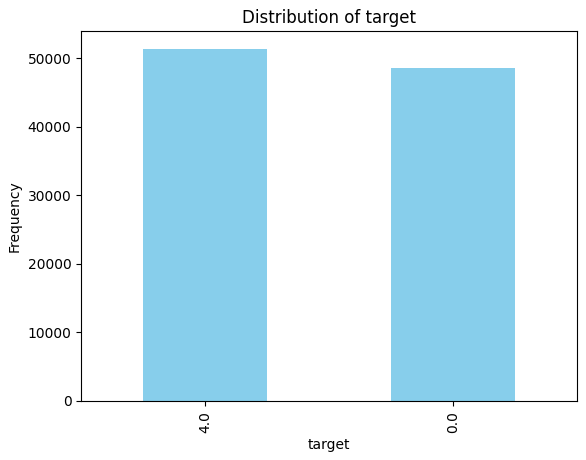
\includegraphics[width=\textwidth]{img/visualize_pic/distribution.png}
    \caption{The Distribution of Target}
\end{figure}

\subsection{Relationships of the Attributes}

Complementing this, the \textbf{Pairwise Relationships} Pairplot provides deeper insights into the numerical features of the dataset, including 'target', 'text\_length', and 'text\_clean\_length'. The histograms show that tweet lengths are typically short, with 'text\_length' peaking between 0–100 characters and 'text\_clean\_length' peaking between 0–40 characters, reflecting the impact of the cleaning process in reducing text length by removing unnecessary characters. Scatter plots reveal no clear correlation between text length (original or cleaned) and sentiment, suggesting that tweet length does not influence sentiment classification. However, a strong linear relationship between 'text\_length' and 'text\_clean\_length' confirms the effectiveness of text cleaning in simplifying the data. Together, these visualizations offer a comprehensive understanding of the dataset’s structure and characteristics, facilitating further analysis and modeling.

\begin{figure}[H]
    \centering
    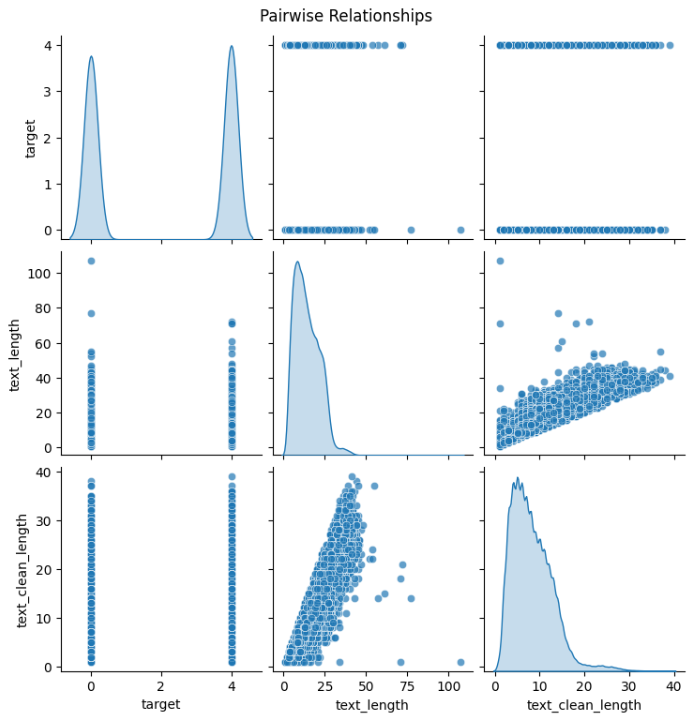
\includegraphics[width=\textwidth]{img/visualize_pic/pairwise.png}
    \caption{Pairwise Relationships}
\end{figure}

\subsection{Top Words Visualizations}

The visual portrayal of the entire dataset showcases the top 20 most frequent words from the 'text\_clean' column, depicted through a graphical chart and a word-based cloud visualization. The chart indicates that 'i' (14,000 occurrences), 'm' (12,000), and 'modi' (10,000) lead in frequency, accompanied by common verbs like 'get,' 'like,' and 'go,' and positive expressions such as 'good,' 'love,' and 'great.' The word-based cloud visualization enhances this by emphasizing high-frequency terms like 'i,' 'm,' and 'modi' with larger, bolder fonts, while presenting smaller fonts for less frequent words like 'great' and 'lol.' Together, these visualizations illuminate the prevailing lexicon in the dataset, highlighting frequent pronouns, verbs, and sentiment-related terms, which reflect the informal tone of Twitter interactions and offer valuable insights into the dataset’s linguistic patterns.

\begin{figure}[H]
    \centering
    \begin{subfigure}[b]{0.48\textwidth}
        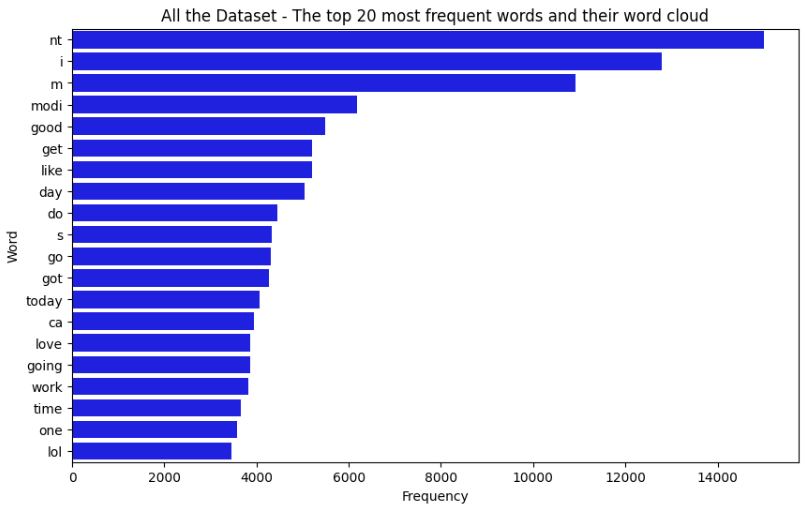
\includegraphics[width=\textwidth]{img/visualize_pic/top20.png}
    \end{subfigure}
    \begin{subfigure}[b]{0.48\textwidth}
        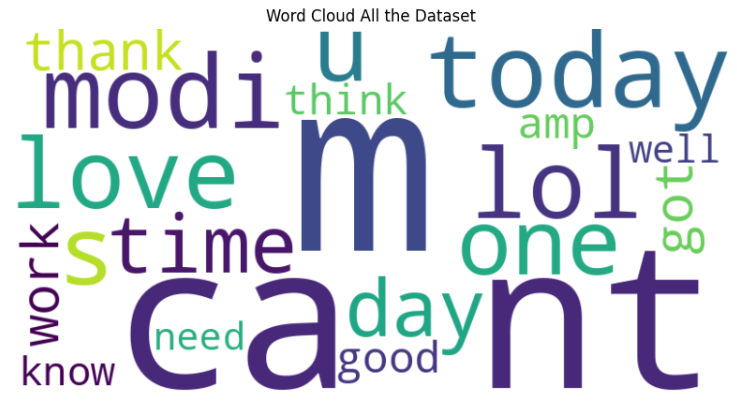
\includegraphics[width=\textwidth]{img/visualize_pic/top20_word_cloud.png}
    \end{subfigure}
    \caption{Top 20 of entire dataset}
\end{figure}

The visualization for the positive class in the sampled dataset is illustrated through the bar chart and word cloud of the top 20 most frequent words from tweets with a 'target' value of 4.0. The bar chart shows that 'i' (5,000 occurrences), 'm' (4,500), and 'modi' (4,000) are the most frequent, followed by positive sentiment words such as 'good' (3,500), 'love' (3,000), 'thanks' (1,800), and 'great' (500), alongside casual terms like 'lol' and 'haha.' The word cloud visually reinforces this, with larger, bolder fonts for high-frequency words like 'i,' 'm,' 'modi,' and 'good,' and smaller fonts for less frequent words like 'haha' and 'great.' These visualizations highlight the linguistic characteristics of positive tweets, emphasizing optimism, gratitude, and humor, which are typical of this sentiment class in the dataset.

\begin{figure}[H]
    \centering
    \begin{subfigure}[b]{0.48\textwidth}
        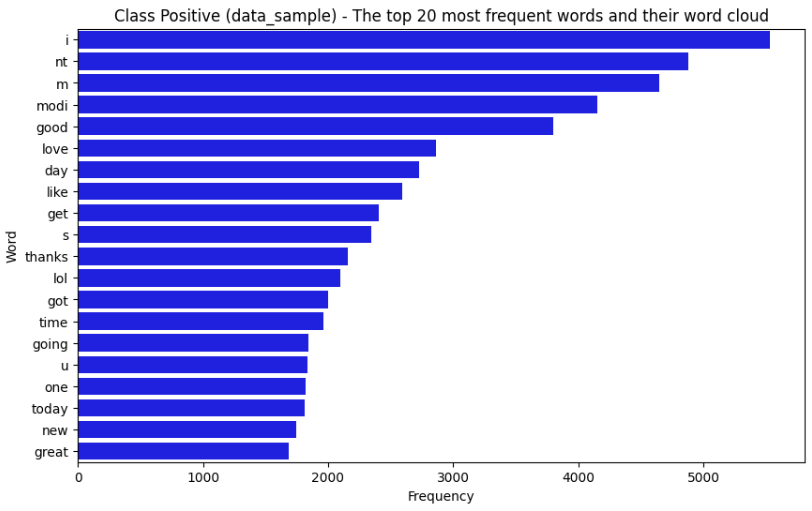
\includegraphics[width=\textwidth]{img/visualize_pic/top20_posi.png}
    \end{subfigure}
    \begin{subfigure}[b]{0.48\textwidth}
        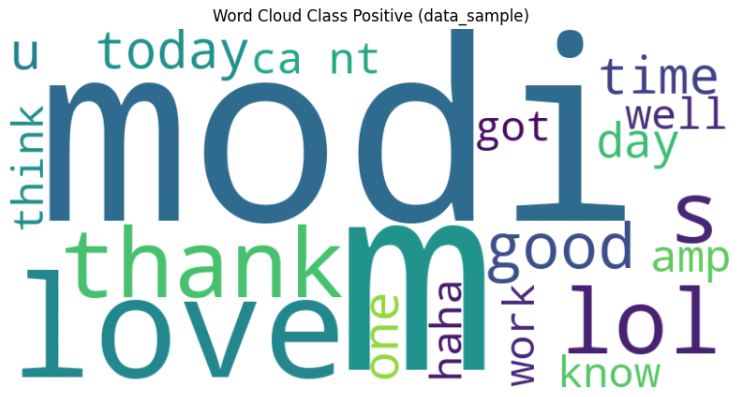
\includegraphics[width=\textwidth]{img/visualize_pic/posi_wordcloud.png}
    \end{subfigure}
    \caption{Top 20 of class Positive}
\end{figure}

The visualization for the negative class in the sampled dataset is depicted through the bar chart and word cloud of the top 20 most frequent words from tweets with a 'target' value of 0.0. The bar chart indicates that 'i' (10,000 occurrences), 'm' (9,000), and 'don’t' (8,000) are the most frequent, followed by words like 'get' (7,000), 'go' (6,000), and 'ca' (5,000), along with negative or frustrated terms such as 'really,' 'want,' 'still,' 'think,' 'need,' and 'miss.' The word cloud visually emphasizes these findings, with larger, bolder fonts for high-frequency words like 'i,' 'm,' 'don’t,' and 'get,' and smaller fonts for less frequent words like 'miss' and 'need.' These visualizations reveal the linguistic patterns of negative tweets, underscoring sentiments of frustration, restriction, and dissatisfaction, which are characteristic of this sentiment class in the dataset.

\begin{figure}[H]
    \centering
    \begin{subfigure}[b]{0.48\textwidth}
        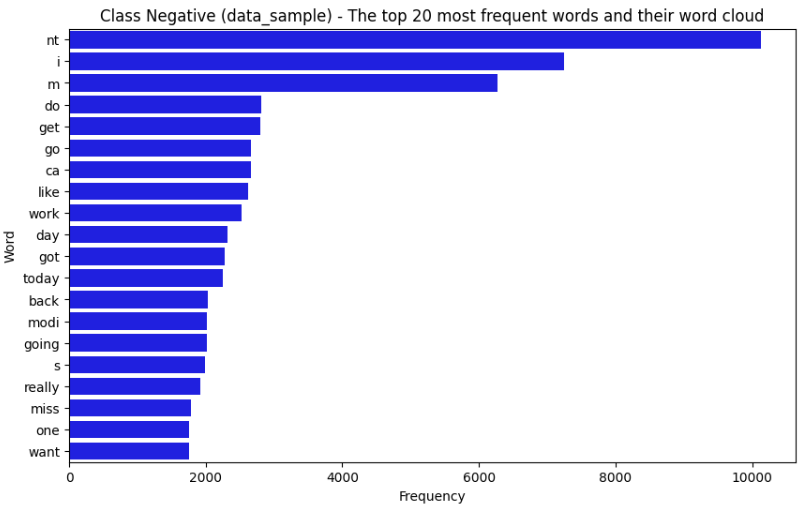
\includegraphics[width=\textwidth]{img/visualize_pic/top20_nega.png}
    \end{subfigure}
    \begin{subfigure}[b]{0.48\textwidth}
        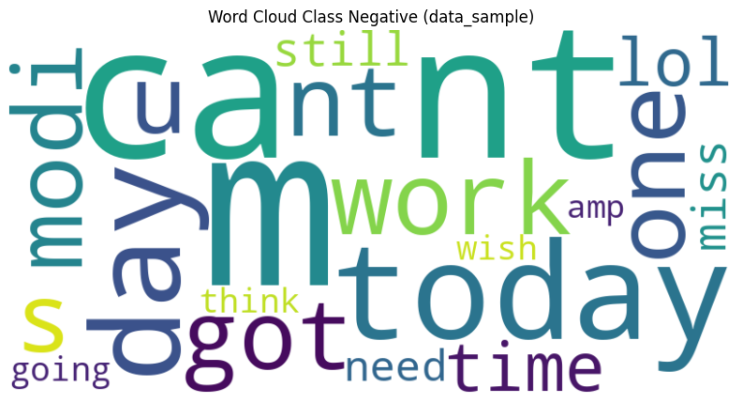
\includegraphics[width=\textwidth]{img/visualize_pic/nega_wordcloud.png}
    \end{subfigure}
    \caption{Top 20 of class Negative}
\end{figure}

\subsection{The distribution of Text Length}

The graphical representations of cleaned tweet lengths (text\_clean\_length) across sentiment classes in the dataset are depicted through a boxplot and histogram. The boxplot indicates that tweets labeled as negative (target = 0.0, in blue) and positive (target = 4.0, in orange) have comparable median lengths, around 10–15 characters, with interquartile ranges extending approximately 5–20 characters. The tighter range (0–40 characters) compared to original text lengths emphasizes the cleaning process’s effect in eliminating unnecessary characters like punctuation and hashtags. Outliers stretching to 35–40 characters are rare and not associated with any particular sentiment, implying that cleaned text length is largely independent of sentiment classification. The histogram complements this by showing that both negative and positive tweets predominantly range between 0 and 10 characters, peaking at about 9,000 for negative tweets and slightly fewer for positive tweets in that range, with frequencies dropping steeply beyond 10 characters and very few tweets surpassing 20 characters. This right-skewed distribution underscores the concise nature of cleaned Twitter data, revealing no significant differences in length distribution between negative and positive sentiments, suggesting that cleaned text length does not play a major role in determining sentiment.

\begin{figure}[H]
    \centering
    \begin{subfigure}[b]{0.48\textwidth}
        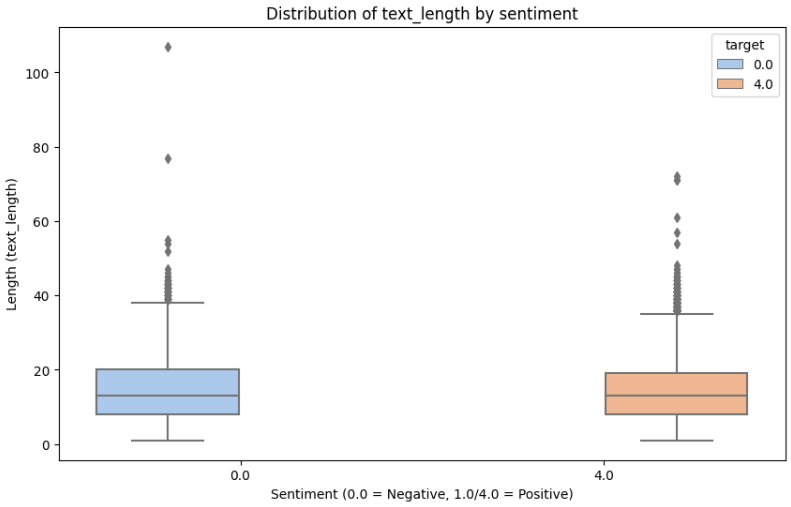
\includegraphics[width=\textwidth]{img/visualize_pic/text_length.png}
    \caption{Distribution of text\_length by sentiment}
    \end{subfigure}
    \begin{subfigure}[b]{0.48\textwidth}
         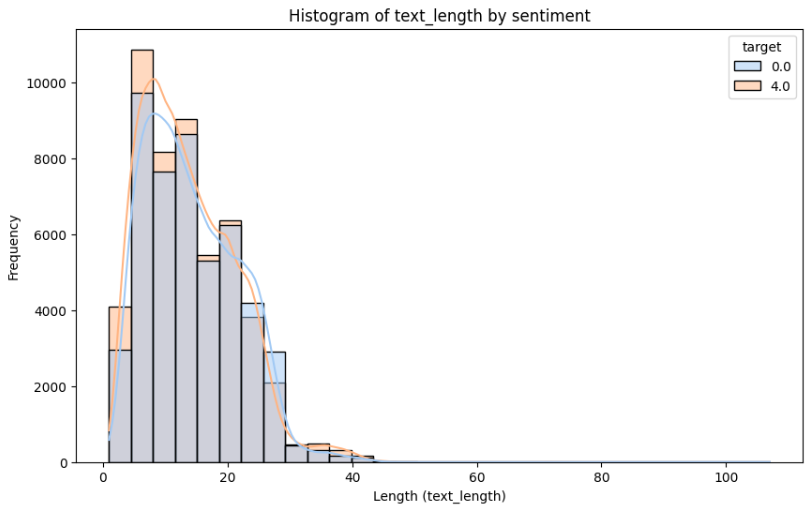
\includegraphics[width=\textwidth]{img/visualize_pic/histogram_text_length.png}
    \caption{Histogram of text\_length by sentiment}
    \end{subfigure}
\end{figure}

The visualizations of cleaned tweet lengths (text\_clean\_length) across sentiment classes in the dataset are illustrated through a boxplot and histogram. The boxplot shows that tweets labeled as negative (target = 0.0, in blue) and positive (target = 4.0, in orange) share similar median lengths, around 10–15 characters, with interquartile ranges spanning roughly 5–20 characters. The narrower range (0–40 characters) compared to original text lengths underscores the cleaning process’s role in removing extraneous characters such as punctuation and hashtags. Outliers reaching up to 35–40 characters are infrequent and not tied to any specific sentiment, indicating that cleaned text length is generally unrelated to sentiment classification. The histogram complements this by revealing that both negative and positive tweets mostly fall between 0 and 10 characters in length, peaking at approximately 9,000 for negative tweets and slightly less for positive tweets in that range, with frequencies declining sharply beyond 10 characters and very few tweets exceeding 20 characters. This right-skewed pattern highlights the concise nature of cleaned Twitter data, showing no notable variation in length distribution between negative and positive sentiments, suggesting that cleaned text length does not significantly affect sentiment determination.

\begin{figure}[H]
    \centering
    \begin{subfigure}[b]{0.48\textwidth}
        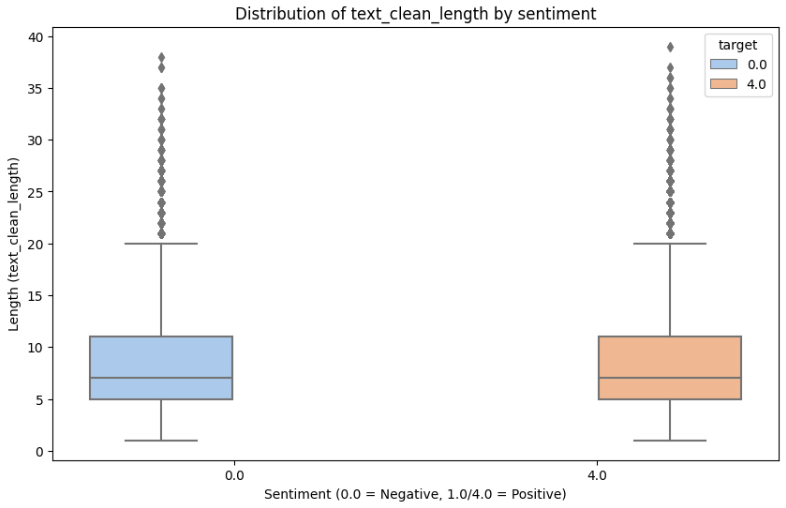
\includegraphics[width=\textwidth]{img/visualize_pic/text_clean.png}
    \caption{Distribution of text\_clean\_length by sentiment}
    \end{subfigure}
    \begin{subfigure}[b]{0.48\textwidth}
         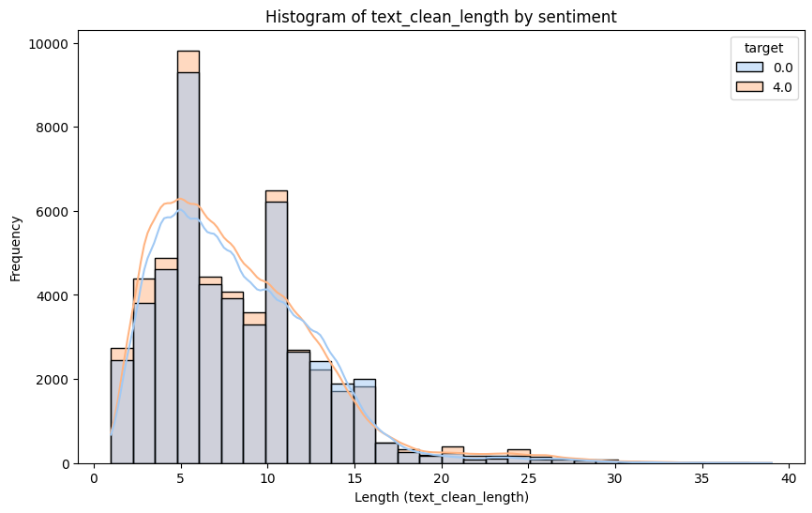
\includegraphics[width=\textwidth]{img/visualize_pic/text_clean_histogram.png}
    \caption{Histogram of text\_clean\_length by sentiment}
    \end{subfigure}
\end{figure}

\subsection{Word Frequencies by Labels}

A heatmap delivers a comprehensive analysis of word frequencies by sentiment, enabling trends to be identified quickly at a glance. It displays the same words—“day,” “going,” “good,” “got,” “like,” “lol,” “love,” “m,” “modi,” “nt,” “s,” “thanks,” “today,” and “work”—with color intensity indicating frequency, ranging from light yellow (representing low frequency, such as 0 occurrences) to dark red (indicating high frequency, for example, 10,130 for “modi” in negative tweets). For instance, “modi” emerges as a prominent term in negative tweets, marked by a deep red shade, while “good” and “love” shine vividly in positive tweets, underscoring their connection to positivity. Together, these representations create a clear and dynamic portrayal of the dataset’s linguistic patterns, emphasizing how word usage mirrors underlying sentiments and providing valuable insights for deeper analysis.

\begin{figure}[H]
    \centering
    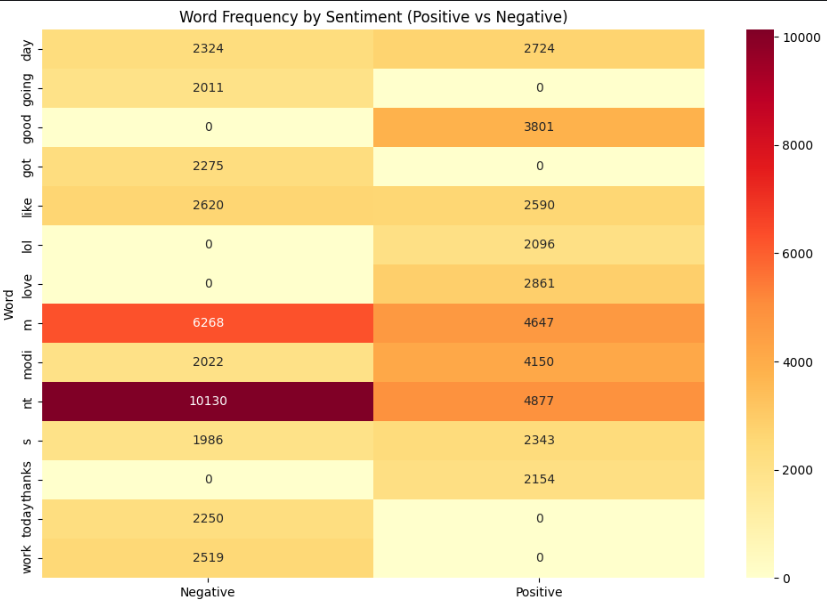
\includegraphics[width=\textwidth]{img/visualize_pic/word_frequency.png}
    \caption{Word Frequency by Sentiment}
\end{figure}

A bar chart provides a straightforward comparison of word frequencies across positive and negative sentiments, illustrating how specific words differ in usage. It shows that terms like “modi” and “m” appear much more frequently in negative tweets, with “modi” recorded around 10,130 times and “m” at 6,268 times, in contrast to 4,877 and 4,647 times in positive tweets, respectively. On the other hand, positive tweets exhibit greater occurrences of words such as “good” (3,801 times) and “love” (2,861 times), which are largely absent or scarce in negative tweets. This striking contrast highlights the unique emotional undertones, with negative tweets often reflecting frustration or limitation, while positive tweets express optimism and warmth.

\begin{figure}[H]
    \centering
    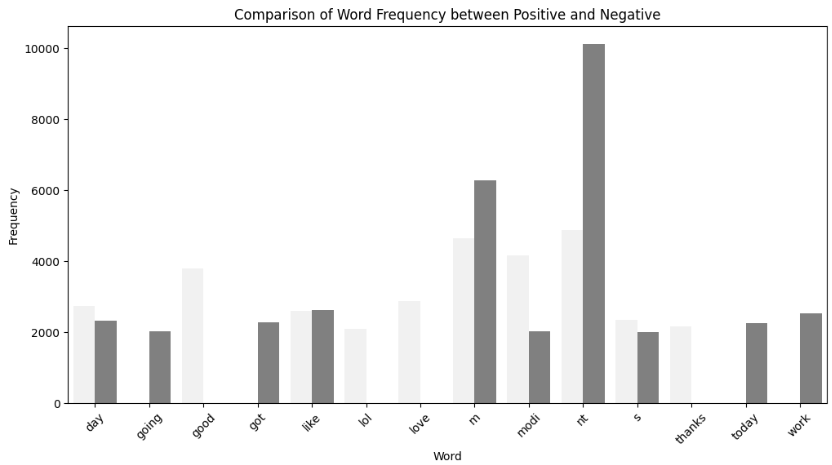
\includegraphics[width=\textwidth]{img/visualize_pic/comparision.png}
    \caption{Comparision of Word Frequency}
\end{figure}

\newpage
